%
% analysis, example programs
%

\chapter{Results}
\label{ch:results}
% \epigraph{Dionysus [is] the Master of Illusions, who could make a vine grow
% out grow out of a ship's plank, and in general enable his votaries to see the
% world as the world's not.}%
% {\textsc{---e.\ r.\ dodds}\\\textit{The Greeks and the Irrational}}

% \epigraph{If the immutable appears recast, then you yourself have been
% transformed.}%
% {\textsc{---r.\ scott bakker}\\\textit{The Judging Eye}}

\epigraph{Logic merely enables one to be wrong with authority}%
{\textsc{---the doctor}} %\\\textit{The Wheel in Space}}

% \begin{itemize}
%     \item performance \& analysis
%     \begin{itemize}
%       \item What is an optimisation? Describe the metrics considered.
%         \begin{itemize}
%           \item wall-clock time, parallel speedup??
%           \item instruction count
%           \item memory traffic (load/store/coalescing)
%           \item memory size (heap, register count, shared memory)
%           \item program size (number of parallel steps)
%           \item code size (generated binary, compilation time c.f. code complexity)
%         \end{itemize}
%     \end{itemize}
%
%     \item expressiveness / example programs
%     \item difficulties
%     \begin{itemize}
%         \item code generation
%         \item unintentional nesting
%     \end{itemize}
% \end{itemize}

The previous chapters discussed the design, implementation and optimisation of
the Accelerate language and CUDA backend. This chapter analyses the performance
of the implementation. Benchmarks were conducted on a single Tesla T10 processor
(compute capability 1.3, 30 multiprocessors = 240 cores at 1.3GHz, 4GB RAM)
backed by two quad core Xeon E5405 CPUs (64-bit, 2GHz, 8GB RAM) running
GNU/Linux (Ubuntu 12.04 LTS, CUDA 5.0).


\section{Runtime Overheads}

Runtime program optimisation, code generation, kernel loading, data transfer,
and so on can contribute significant overhead to short lived GPU computations.
Accelerate mitigates these overheads via caching and memoisation. For example,
the first time a particular expression is executed it is compiled to CUDA code,
which is reused for subsequent invocations. This section analyses those
overheads, so that they can be factored out later when we discuss the effects of
the program optimisations on kernel runtimes of the benchmark programs.


\subsection{Program Optimisation}

% tk: performance and benchmarks for the fusion pass
%   - actual runtime
%   - tick counters for the final version and old one with extend/cunctation
%     separation

\subsection{Data Transfer}

% tk: some graphs of memory transfer times or bandwith vs. array size
% tk: importance of using weak pointers, so data transfers ``escape'' the black
%     box of evaluating the AST --> hashcat.
% tk: importance of the nursery for reducing calls to malloc/free

\subsection{Code Generation \& Compilation}

% tk: measure \& tabulate some code generation / compilation times
% tk: persistent cache, perhaps just a mention?


\section{Dot product}

Dot product, or scalar product, is an algebraic operation that takes two
equal-length sequences of numbers and returns a single number by computing the
sum of the products of the corresponding entries in the two sequences. Dot
product can be defined in Accelerate using the code below, which was also seen
in section~\ref{sec:producer_consumer_fusion}.
%
\begin{lstlisting}[style=haskell
    ,label=lst:dotp
    ,caption={Vector dot-product in Accelerate}]
dotp :: Acc (Vector Float) -> Acc (Vector Float) -> Acc (Scalar Float)
dotp xs ys = A.fold (+) 0                       -- sum result of\ldots
           $ A.zipWith (*) xs ys                -- \ldots element-wise multiplying inputs
\end{lstlisting}
%
Figure~\ref{fig:dotp} show the result of running this code, compared to several
other sequential and parallel implementations. The \texttt{Data.Vector} baseline
is sequential code produced by \index{fusion!stream}stream
fusion~\cite{Coutts:2007kp}, running on the host CPU. The \texttt{Repa} version
runs in parallel on all eight cores of the host CPU, using the fusion method of
\index{fusion!delayed arrays}delayed arrays~\cite{Keller:2010er}. The
\texttt{NDP2GPU}~\cite{Bergstrom:2012bi} version compiles NESL
code~\cite{Blelloch:1995ut} down to CUDA. The performance of this version
suffers because the \texttt{NDP2GPU} compiler uses the legacy NESL compiler for
the front-end, which introduces redundant administrative operations that are not
strictly needed when evaluating a dot product.

\begin{figure}[htbp]
    \begin{center}
        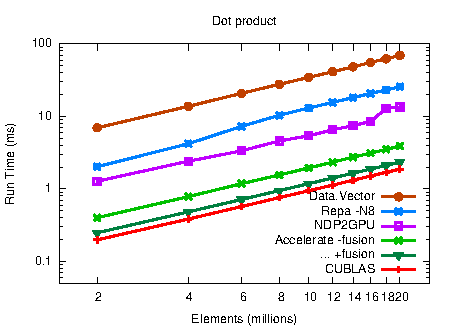
\includegraphics[width=0.8\textwidth]{images/sec-6/dotp/dotp}
    \end{center}
    \caption[Vector dot product kernel benchmarks]{Kernel runtimes for vector
        dot product, in Accelerate with and without optimisations, compared to
        other parallel GPU and CPU implementations. Note the log-log scale.}
    \label{fig:dotp}
\end{figure}

Without optimisations the Accelerate version executes in approximately twice the
time of the CUBLAS version. Since the individual aggregate operations consist of
only a single arithmetic operation each, the problem can not be a lack of
sharing.


\subsection{Too many kernels}

The slow-down in the unoptimised version is due to Accelerate generating one GPU
kernel function for each aggregate operation in the source program. The use of
two separate kernels requires the intermediate array produced by \code{zipWith}
to be constructed in GPU memory before being immediately read back by
\code{fold}. In contrast the CUBLAS version uses only a single kernel. As this
is a simple memory bound benchmark, lack of fusion roughly doubles the runtime.

The fused version of dot product combines the aggregate computations by
embedding a function of type \code{(sh -> a)} into the reduction, represented
here as the second argument to the constructor \code{Delayed}. This scalar
function does the work of element wise multiplying the two input vectors, and is
performed on-the-fly as part of the reduction kernel instead of requiring an
intermediate array:
%
\begin{lstlisting}[style=haskell]
let a0 = use (Array ...) in
let a1 = use (Array ...) in
fold (\x0 x1 -> x0 + x1) 0.0
   (Delayed (intersect (shape a0) (shape a1))   -- extent of the input array
            (\x0 -> (a0!x0) * (a1!x0)))         -- function to generate a value at each index
\end{lstlisting}

While the fused Accelerate version is $30\times$ faster than the sequential
version executed on the CPU, it is still approximately $20\%$ slower than the
hand-written CUBLAS version. As dot product is a computationally simple task,
any additional overheads in the implementation will be significant. To see why
this version is still slightly slower, we analyse the generated code to inspect
it for sources of overhead.


\subsection{Duplicate loop counters}

The fused dot product operation will only perform the element wise
multiplication of the two input arrays in the first step of the tree reduction
(\S\ref{sec:parallel_reduction}). This occurs in the phase of the cascaded
algorithm when individual threads sequentially sum multiple elements. After
embedding the fused producer, the following CUDA code is generated for the inner
loop of this step:
%
% pookie is the bestest
% bubbaboo ish silly
% kekekee
% i can't put smiley faces in cause weird things happen
% hehe^{this is my thesis
% please like it
% i worked really hard
% and writed a lots
% }<++>
%
%
\begin{lstlisting}[style=cuda
    ,firstnumber=18
    ,label=lst:dotp_cuda
    ,caption={Generated CUDA code for the first step of fused dot product}]
for (ix += gridSize; ix < shapeSize; ix += gridSize) {
    const Int64 v2 = ix;
    const int v3 = toIndex(shIn0, shape(v2));
    const int v4 = toIndex(shIn1, shape(v2));

    x0 = arrIn0_a0[v3] * arrIn1_a0[v4];
    y0 = x0 + y0;
}
\end{lstlisting}
%
We have four loop counters: \code{ix}, \code{v2}, \code{v3} and \code{v4} ---
two for the source arrays and two to convert between the multidimensional and
linear representations. These counters contain the same value and are
incremented in lockstep. In addition to the superfluous arithmetic, the
duplication of counters unnecessarily increases register pressure.

\marginnote{this was unexpected}
The corresponding section of PTX~\cite{NVIDIA:2012vj} code is for this loop is
shown in Listing~\ref{lst:dotp_ptx}. To retrieve the data from the first input
array, the input array pointer is retrieved (line~\ref{lst:dotp_ptx_ldparam}),
the offset stored in register \code{rd16} added to it
(line~\ref{lst:dotp_ptx_add}), and then the value read from global memory at
this address (line~\ref{lst:dotp_ptx_ldglobal}). Happily, we note that
retrieving the second input element \emph{also} uses the offset stored in
register \code{rd16} (line~\ref{lst:dotp_ptx_ldglobal2}).
%
\begin{lstlisting}[style=ptx
    ,float
    ,firstnumber=103
    ,label=lst:dotp_ptx
    ,caption={Corresponding PTX code for the first step of fused dot product}]
 //  18          for (ix += gridSize; ix < shapeSize; ix += gridSize) {
        cvt.u32.u16     %r10, %nctaid.x;
        mul.lo.u32      %r11, %r10, %r1;
        add.s32         %r12, %r11, %r7;
        mov.s32         %r13, %r12;
        setp.le.s32     %p2, %r8, %r12;
        @%p2 bra        $Lt_0_13058;
        cvt.s64.s32     %rd12, %r12;
        cvt.s64.u32     %rd13, %r11;
$Lt_0_14082:
 //<loop> Loop body line 18, nesting depth: 1, estimated iterations: unknown
        .loc    16      24      0
 //  20              const int v3 = toIndex(shIn0, shape(v2));
 //  21              const int v4 = toIndex(shIn1, shape(v2));
 //  22
 //  23              x0 = arrIn0\_a0[v3] * arrIn1\_a0[v4];
 //  24              y0 = x0 + y0;
        cvt.s32.s64     %rd14, %rd12;                           (@* \label{lst:dotp_ptx_cvt1} *@)
        cvt.s32.s64     %r14, %rd14;
        cvt.s64.s32     %rd15, %r14;                            (@* \label{lst:dotp_ptx_cvt3} *@)
        mul.wide.s32    %rd16, %r14, 4;
        .loc    16      17      0
        ld.param.u64    %rd9, [__cudaparm_foldAll_arrIn0_a0];   (@* \label{lst:dotp_ptx_ldparam} *@)
        .loc    16      24      0
        add.u64         %rd17, %rd16, %rd9;                     (@* \label{lst:dotp_ptx_add} *@)
        ld.global.f32   %f4, [%rd17+0];                         (@* \label{lst:dotp_ptx_ldglobal} *@)
        .loc    16      17      0
        ld.param.u64    %rd8, [__cudaparm_foldAll_arrIn1_a0];
        .loc    16      24      0
        add.u64         %rd18, %rd16, %rd8;
        ld.global.f32   %f5, [%rd18+0];                         (@* \label{lst:dotp_ptx_ldglobal2} *@)
        mad.f32         %f3, %f4, %f5, %f3;
        add.s32         %r13, %r13, %r11;
        add.s64         %rd12, %rd12, %rd13;
        setp.gt.s32     %p3, %r8, %r13;
        @%p3 bra        $Lt_0_14082;
        bra.uni         $Lt_0_13058;
$Lt_0_13314:
        mov.f32         %f3, %f6;
$Lt_0_13058:
        .loc    16      27      0
 //  25          }
\end{lstlisting}

In this case the CUDA compiler was able to coalesce our four counters into a
single counter. This is because our definition of \code{toIndex} specialised for
one-dimensional indices \code{DIM1} does \emph{not} do bounds checking:
%
\begin{lstlisting}[style=cuda]
template <>
static __inline__ __device__ Ix toIndex(const DIM1 sh, const DIM1 ix)
{
    return ix;
}
\end{lstlisting}
%
Since we do not check that the current index \code{ix} is within bounds of the
array shape \code{sh}, the compiler can see that the definitions of \code{v3}
and \code{v4} in Listing~\ref{lst:dotp_cuda} are identical. Similarly
one-dimensional indices are just integers, and so the one-dimensional instance
of \code{shape} is the identity function. For higher dimensional shapes,
however, this is not the case and \code{toIndex} and \code{shape} do real work
to their arguments. As the shape \code{shIn0} and \code{shIn1} are inputs
arguments to the kernel, the compiler will not be able to determine they are
equivalent and so the counters would not be combined.

Why don't we perform bounds checks in \code{toIndex}? Implementing exceptions in
a massively parallel architecture is difficult, and support for throwing
exceptions from kernel functions was only recently added for devices of compute
capability 2.0 and later~\cite{NVIDIA:2012wf}. % [\SB.15]
It would be a straightforward matter of adding runtime bounds checks for
supported devices, however.


\subsection{64-bit Arithmetic}

CUDA devices are at their core 32-bit processors and thus are optimised for
32-bit arithmetic. For example, our Tesla GPU with compute capability 1.3 has a
throughput of eight 32-bit floating-point add, multiply, or multiply-add
operations per clock cycle per multiprocessor, but only a single operation per
cycle of the 64-bit equivalents of these~\cite{NVIDIA:2012wf}. % [\S5.4.1]

However, the host architecture that the Haskell program executes on is likely to
be a 64-bit processor. This means that an \code{Int} value from Haskell ---
which may appear marshalled as array data or shape values --- will generate code
to manipulate 64-bit integers, as well as conversions between 32- and 64-bit
types. Lines~\ref{lst:dotp_ptx_cvt1}--\ref{lst:dotp_ptx_cvt3} of
Listing~\ref{lst:dotp_ptx} contain such type conversions, which on our compute
capability 1.3 device have a throughput of only a single operation per cycle per
multiprocessor. These conversions would not be necessary if we were not
cross-compiling from a 64-bit Haskell host, or if the programmer working
directly with CUDA only used the \code{int} type, which would be interpreted by
the CUDA compiler as a 32-bit wide integer.


\subsection{Non-neutral starting elements}

For convenience, and to avoid possibly unexpected behaviour, Accelerate's
\code{fold*} family of functions do not require the combination function and
starting element to form a moniod. We still require the function to be
associative, so that the reduction can be implemented efficiently in parallel as
a tree-reduction, but the initial element does not need to be a \emph{neutral}
element.\marginnote{semigroup?} For example, \code{fold (+) 10} is valid in
Accelerate and evaluates to the correct answer.

However, this means that evaluation of the reduction is more complex. In
particular, we can not simply initialise all threads to the initial value.
In the first phase of the reduction, threads must be sure to initialise
their local sum \code{y0} with values from the input array before beginning the
sequential loop show in Listing~\ref{lst:dotp_cuda}:
%
% tk: hacks in comment style below: check if changing the basic language style
\begin{lstlisting}[style=cuda,firstnumber=12]
if (ix < shapeSize) {
    const Int64 v2 = ix;
    const int v3 = toIndex(shIn0, shape(v2));
    const int v4 = toIndex(shIn1, shape(v2));

    y0 = arrIn0_a0[v3] * arrIn1_a0[v4];
    for (ix += gridSize; ix < shapeSize; ix += gridSize) {
\end{lstlisting}

Similarly, in the second parallel tree reduction phase threads may only read
values from shared memory that were properly initialised. This requires
additional bounds checks at every step:
%
\begin{lstlisting}[style=cuda,firstnumber=27]
sdata0[threadIdx.x] = y0;
__syncthreads();
ix = min(shapeSize - blockIdx.x * blockDim.x, blockDim.x);
if (threadIdx.x + 512 < ix) {
    x0 = sdata0[threadIdx.x + 512];
    y0 = y0 + x0;
    sdata0[threadIdx.x] = y0;
}
__syncthreads();
if (threadIdx.x + 256 < ix) {
    x0 = sdata0[threadIdx.x + 256];
    y0 = y0 + x0;
    sdata0[threadIdx.x] = y0;
}
__syncthreads();
// etc...
\end{lstlisting}

These requirements increase overhead from ancillary instructions that are not
loads, stores, or arithmetic for the core computation. A summation reduction has
low arithmetic intensity to begin with, and is the limiting factor in the
performance of this kernel, so additional bounds checks further reduce
performance.

\subsection{Kernel Specialisation}

To further reduce instruction overhead, it is possible to completely unroll the
reduction by specialising the kernel for a specific block size. In standard CUDA
this can be achieved through the use of C++ templates. Branches referring to the
template parameter will be evaluated at compile time, resulting in a very
efficient inner loop.
%
\begin{lstlisting}[style=cuda]
template <unsigned int blockSize> __global__ void reduce(...) {
    ...
    if (blockSize > 512) {
    }
    if (blockSize > 256) {
    }
    ...
\end{lstlisting}

This technique has shown to produce significant gains in
practice~\cite{Harris:2007te}, although requires compiling a separate kernel for
each thread block size we wish to specialise for. Accelerate can achieve this
kind of kernel specialisation because the CUDA code is generated at program
runtime, but this extra compilation adds significant additional overhead. Since
compiled kernels are cached and reused (\S tk), if we know that the reduction
will be computed many times the extra compilation overhead can be amortised by
the improved kernel performance, and may thus be worthwhile. Such
specialisations are left for future work.


\section{Black-Scholes option pricing}

The Black-Scholes algorithm is a partial differential equation for modelling the
evolution of a European-style stock option price under certain assumptions. The
corresponding Accelerate program is shown in Listing~\ref{lst:blackscholes}.
Given a vector of triples of the underlying stock price, strike price, and time
to maturity in years, the Black-Scholes formula computes the price of a call and
put option. The function \code{callput} evaluates the Black-Scholes formula for
a single triple, and \code{blackscholes} maps it over a vector of triples such
that all individual applications of the formula are executed in parallel.
%
\begin{lstlisting}[style=haskell
    ,float
    ,label=lst:blackscholes
    ,caption={Black-Scholes option pricing in Accelerate}]
horner :: Num a => [a] -> a -> a
horner coeff x =
  let madd a b  = a + x*b
  in
  x * foldr1 madd coeff

cnd' :: Floating a => a -> a
cnd' d =
  let poly      = horner coeff
      coeff     = [0.31938153,-0.356563782,1.781477937,-1.821255978,1.330274429]
      rsqrt2pi  = 0.39894228040143267793994605993438
      k         = 1.0 / (1.0 + 0.2316419 * abs d)
  in
  rsqrt2pi * exp (-0.5*d*d) * poly k

blackscholes :: Acc (Vector (Float, Float, Float)) -> Acc (Vector (Float, Float))
blackscholes = A.map callput
  where
  callput x =
    let (price, strike, years) = A.unlift x
        r       = A.constant riskfree
        v       = A.constant volatility
        v_sqrtT = v * sqrt years
        d1      = (log (price / strike) + (r + 0.5 * v * v) * years) / v_sqrtT
        d2      = d1 - v_sqrtT
        cnd d   = let c = cnd' d in d >* 0 ? (1.0 - c, c)
        cndD1   = cnd d1
        cndD2   = cnd d2
        x_expRT = strike * exp (-r * years)
    in
    A.lift ( price * cndD1 - x_expRT * cndD2                    -- call price
           , x_expRT * (1.0 - cndD2) - price * (1.0 - cndD1))   -- put price
\end{lstlisting}

Figure~\ref{fig:blackscholes} shows the result of running this code compared to
the implementation that ships with the CUDA SDK. Without optimisations, the
Accelerate version is almost twenty times slower than the equivalent
implementation in CUDA C. As \code{blackscholes} includes only one collective
array operation, the problem can not be a lack of fusion.

\begin{figure}[htbp]
    \begin{center}
        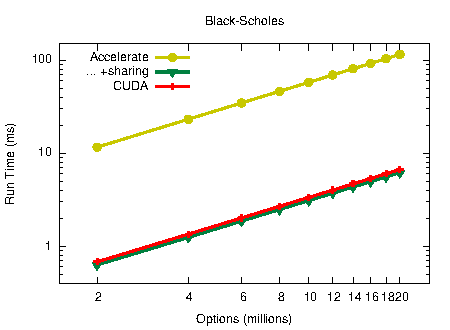
\includegraphics[width=0.8\textwidth]{images/sec-6/black-scholes/black-scholes}
    \end{center}
    \caption[Black-Scholes kernel benchmarks]{Kernel runtimes for Black-Scholes
        options pricing, in Accelerate with and without optimisations, compared
        to a hand-written CUDA version. Note the log-log scale.}
    \label{fig:blackscholes}
\end{figure}

\subsection{Too little sharing}

The function \code{callput} from Listing~\ref{lst:blackscholes} includes a
significant amount of sharing: the helper functions \code{cnd'} and hence
\code{horner} are used twice --- for \code{d1} and \code{d2} --- and its
argument \code{d} is used multiple times in the body. Furthermore, the
conditional expression \code{d >* 0 ? (1 - c, c)} results in a branch that,
without sharing, results in a growing number of predicated instructions that
leads to a large penalty on the SIMD architecture of the GPU.

Without sharing the generated code requires 2573 instructions and results in
\marginnote{check instruction count difference}
significant warp divergence which serialises portions of the execution. With
sharing recovery the generate code requires 501 instructions and is actually
slightly faster than the reference CUDA version because the latter contains a
common subexpression that is not spotted by the programmer and not eliminated by
the CUDA compiler. The common subexpression performs a single multiplication.

